\chapter{Случайные величины и распределения}\label{chap:random-variables}\markright{Глава 37}

\section{Случайная величина и её распределение}
\begin{definition}\term{Случайная величина} (\emph{random variable}) — функция \(X:\Omega\to\mathbb R\), для которой \(\{\omega:X(\omega)\le t\}\) является событием при каждом \(t\in\mathbb R\). \par\term{Измеримость} (\emph{measurability}) — выполнение этого условия отображением \(X\).\end{definition}
\begin{definition}\term{Функция распределения} (\emph{cumulative distribution function, CDF}) величины \(X\) есть \(F_X(t)=\mathbb P(X\le t)\). \par\term{Дискретная случайная величина} (\emph{discrete random variable}) принимает конечное или счётное множество значений \(x_j\) с вероятностями \(p_j\), причём \(\sum_jp_j=1\).\end{definition}
\begin{definition}\term{Плотность вероятности} (\emph{probability density}) — неотрицательная интегрируемая функция \(f_X\), для которой \(F_X(t)=\int_{-\infty}^t f_X(x)\,dx\) и \(\int_{-\infty}^{\infty}f_X(x)\,dx=1\). \par\term{Абсолютно непрерывная случайная величина} (\emph{absolutely continuous random variable}) — случайная величина с плотностью вероятности. Здесь достаточно обычных несобственных интегралов; общая теория меры шире этой модели.\end{definition}
\par\addvspace{5pt}\begin{lrbox}{\CatFlowBox}\begin{minipage}[t]{\linewidth}
\setlength{\parskip}{5pt}\setlength{\columnsep}{4.5mm}\setlength{\intextsep}{0pt}
\begin{wrapfigure}[9]{r}{54mm}

\includegraphics[width=54mm,height=58mm,keepaspectratio]{images/unique/art-172.png}
\end{wrapfigure}
Плотность сама не является вероятностью точки. Вероятность интервала равна площади под графиком плотности; значение плотности может даже превышать единицу на коротком промежутке. У дискретной величины вероятность сосредоточена в отдельных значениях, а её функция распределения имеет скачки. Распределения бывают и смешанными, поэтому деление на дискретные и имеющие плотность не исчерпывает всех случаев.
\par\WFclear\end{minipage}\end{lrbox}%
\ifdim\dimexpr\ht\CatFlowBox+\dp\CatFlowBox\relax<64mm\dp\CatFlowBox=\dimexpr64mm-\ht\CatFlowBox\relax\fi%
\noindent\usebox{\CatFlowBox}\par\addvspace{5pt}
\begin{theorem}[Вероятности через функцию распределения]
Для \(a<b\) выполнено \(\mathbb P(a<X\le b)=F_X(b)-F_X(a)\). Функция \(F_X\) не убывает. Если у \(X\) есть плотность, то \(\mathbb P(X=t)=0\) для каждого \(t\), а включение концов интервала не меняет его вероятности.
\end{theorem}
\begin{proof}Событие \(\{X\le b\}\) разбивается на \(\{X\le a\}\) и \(\{a<X\le b\}\). Отсюда формула и монотонность. При наличии плотности интеграл по одноточечному отрезку равен нулю. Это также следует из непрерывности первообразной интеграла: у \(F_X\) нет скачков.\end{proof}
\section{Среднее, дисперсия и совместные величины}
\begin{definition}\term{Математическое ожидание} (\emph{expected value, expectation}) задаётся формулами
\[
\mathbb EX=\sum_j x_jp_j\quad\hbox{или}\quad
\mathbb EX=\int_{-\infty}^{\infty}x f_X(x)\,dx.
\]
В этой главе ожидание считается существующим как конечное число при абсолютной сходимости: \(\sum_j|x_j|p_j<\infty\) или \(\int |x|f_X(x)\,dx<\infty\). Для измеримой \(g\) и абсолютно интегрируемой \(g(X)\) заменяем \(x\) на \(g(x)\).\end{definition}
\begin{definition}\term{Дисперсия} (\emph{variance}) \(\operatorname{Var}X=\mathbb E(X-\mathbb EX)^2\), если второй момент конечен. \par\term{Среднеквадратическое отклонение} (\emph{standard deviation}) \(\sigma_X=\sqrt{\operatorname{Var}X}\).\end{definition}
\begin{definition}\term{Совместное распределение} (\emph{joint distribution}) описывает пару \((X,Y)\); в конечной модели это числа \(p_{ij}=\mathbb P(X=x_i,Y=y_j)\). \par\term{Независимые случайные величины} (\emph{independent random variables}) удовлетворяют \(\mathbb P(X\in A,Y\in B)=\mathbb P(X\in A)\mathbb P(Y\in B)\) для любых борелевских множеств \(A,B\); борелевские множества получаются из открытых счётными операциями объединения и дополнения.\end{definition}
\begin{definition}\term{Ковариация} (\emph{covariance}) при конечных вторых моментах есть \(\operatorname{Cov}(X,Y)=\mathbb E[(X-\mathbb EX)(Y-\mathbb EY)]\).\end{definition}
\begin{theorem}[Линейность и дисперсия]
Для интегрируемых величин \(\mathbb E(aX+bY+c)=a\mathbb EX+b\mathbb EY+c\). При конечных вторых моментах
\[
\operatorname{Var}X=\mathbb EX^2-(\mathbb EX)^2,\qquad
\operatorname{Var}(aX+b)=a^2\operatorname{Var}X,
\]
\[
\operatorname{Var}(X+Y)=\operatorname{Var}X+\operatorname{Var}Y+2\operatorname{Cov}(X,Y).
\]
Если \(X,Y\) независимы, то \(\operatorname{Cov}(X,Y)=0\).
\end{theorem}
\begin{proof}В конечной модели \(\mathbb E(X+Y)=\sum_{ij}(x_i+y_j)p_{ij}=\sum_i x_i\sum_jp_{ij}+\sum_jy_j\sum_ip_{ij}\). Так же выносятся константы. При абсолютно сходящихся суммах и интегралах рассуждение сохраняется по линейности; для совместной плотности применяется теорема Фубини. Раскрытие квадратов даёт все формулы дисперсии. При независимости совместные вероятности или плотности раскладываются в произведение и \(\mathbb E(XY)=\mathbb EX\mathbb EY\). Для общих измеримых распределений те же свойства доказываются через приближение простыми функциями; здесь используем конечные, счётные и имеющие совместную плотность модели.\end{proof}
\par\addvspace{5pt}\begin{lrbox}{\CatFlowBox}\begin{minipage}[t]{\linewidth}
\setlength{\parskip}{5pt}\setlength{\columnsep}{4.5mm}\setlength{\intextsep}{0pt}
\begin{wrapfigure}[11]{l}{54mm}

\includegraphics[width=54mm,height=58mm,keepaspectratio]{images/unique/art-173.png}
\end{wrapfigure}
Математическое ожидание описывает средний результат большого числа повторений, а дисперсия — масштаб разброса. Одинаковое среднее не означает одинаковое распределение. Результаты \(0,2\) с равными вероятностями и постоянный результат \(1\) имеют одно среднее, но разные дисперсии. При смене единиц измерения среднее масштабируется линейно, а дисперсия — с квадратом коэффициента.
\par\WFclear\end{minipage}\end{lrbox}%
\ifdim\dimexpr\ht\CatFlowBox+\dp\CatFlowBox\relax<64mm\dp\CatFlowBox=\dimexpr64mm-\ht\CatFlowBox\relax\fi%
\noindent\usebox{\CatFlowBox}\par\addvspace{5pt}
\section{Основные распределения}
\begin{definition}\term{Распределение Бернулли} (\emph{Bernoulli distribution}) \(\operatorname{Bern}(p)\), \(0\le p\le1\), задаёт \(X=1\) с вероятностью \(p\) и \(X=0\) с вероятностью \(1-p\). \par\term{Биномиальное распределение} (\emph{binomial distribution}) \(\operatorname{Bin}(n,p)\) — число успехов в \(n\) независимых испытаниях Бернулли.\end{definition}
\begin{theorem}[Среднее и дисперсия числа успехов]
Для \(X\sim\operatorname{Bern}(p)\): \(\mathbb EX=p\), \(\operatorname{Var}X=p(1-p)\). Для \(S\sim\operatorname{Bin}(n,p)\): \(\mathbb ES=np\), \(\operatorname{Var}S=np(1-p)\).
\end{theorem}
\begin{proof}Для индикатора \(X^2=X\), поэтому \(\mathbb EX=\mathbb EX^2=p\). Число успехов есть сумма \(n\) независимых индикаторов. Складываем ожидания и дисперсии.\end{proof}
\begin{definition}\term{Геометрическое распределение} (\emph{geometric distribution}) \(\operatorname{Geom}(p)\), \(0<p<1\), задаёт номер первого успеха: \(\mathbb P(X=k)=(1-p)^{k-1}p\), \(k=1,2,\ldots\). Его среднее \(1/p\), дисперсия \((1-p)/p^2\). При \(p=1\) величина равна \(1\).\end{definition}
\begin{definition}\term{Распределение Пуассона} (\emph{Poisson distribution}) \(\operatorname{Pois}(\lambda)\), \(\lambda>0\), имеет \(\mathbb P(X=k)=e^{-\lambda}\frac{\lambda^k}{k!}\), \(k\in\mathbb N_0\). Его среднее и дисперсия равны \(\lambda\).\end{definition}
Для геометрического закона положим \(q=1-p\). Ряды с членами \(kq^{k-1}\) и \(k(k-1)q^{k-1}\) сходятся по признаку отношений. Обозначив их суммы \(A,B\), вычтем из каждой сумму, умноженную на \(q\), со сдвигом индекса: \((1-q)A=\sum_{k=0}^\infty q^k=1/(1-q)\), \((1-q)B=2qA\). Поэтому \(\mathbb EX=pA=1/p\), \(\mathbb E[X(X-1)]=pB=2q/p^2\), откуда следует дисперсия. Для Пуассона нормировка следует из доказанного в главе о рядах разложения экспоненты; сдвиг индексов даёт \(\mathbb EX=\lambda\), \(\mathbb E[X(X-1)]=\lambda^2\), затем \(\operatorname{Var}X=\lambda\).
\begin{definition}\term{Равномерное распределение} (\emph{uniform distribution}) \(\operatorname U[a,b]\), \(a<b\), имеет плотность \(\frac1{b-a}\) на \([a,b]\) и \(0\) вне него. \par\term{Показательное распределение} (\emph{exponential distribution}) \(\operatorname{Exp}(\lambda)\), \(\lambda>0\), имеет плотность \(\lambda e^{-\lambda x}\) при \(x\ge0\) и \(0\) при \(x<0\).\end{definition}
\begin{theorem}[Моменты двух непрерывных распределений]
Для \(X\sim\operatorname U[a,b]\): \(\mathbb EX=\frac{a+b}2\), \(\operatorname{Var}X=\frac{(b-a)^2}{12}\). Для \(Y\sim\operatorname{Exp}(\lambda)\): \(\mathbb EY=\frac1\lambda\), \(\operatorname{Var}Y=\frac1{\lambda^2}\).
\end{theorem}
\begin{proof}Интегрирование \(x/(b-a)\), \(x^2/(b-a)\) даёт \(\mathbb EX=(a+b)/2\), \(\mathbb EX^2=(a^2+ab+b^2)/3\); вычитаем квадрат среднего. Для показательного закона два интегрирования по частям дают \(\mathbb EY=1/\lambda\), \(\mathbb EY^2=2/\lambda^2\). Граничные члены исчезают, поскольку экспонента убывает быстрее степеней.\end{proof}
\begin{definition}\term{Нормальное распределение} (\emph{normal, Gaussian distribution}) \(\operatorname N(\mu,\sigma^2)\), \(\mu\in\mathbb R,\sigma>0\), имеет плотность
\[
 f_X(x)=\frac1{\sigma\sqrt{2\pi}}\exp\!\left(-\frac{(x-\mu)^2}{2\sigma^2}\right).
\]
\term{Стандартное нормальное распределение} (\emph{standard normal distribution}) — \(\operatorname N(0,1)\); его функция распределения обозначается \(\Phi\).\end{definition}
Нормировка нормальной плотности получается из гауссова интеграла \(\int_{-\infty}^\infty e^{-t^2}\,dt=\sqrt\pi\) заменой переменной; вывод гауссова интеграла дан в задачах главы о кратных интегралах. Нечётность \(z e^{-z^2/2}\) даёт \(\mathbb EZ=0\), интегрирование по частям даёт \(\mathbb EZ^2=1\). Поэтому для \(X=\mu+\sigma Z\) среднее равно \(\mu\), дисперсия — \(\sigma^2\).
\section{Оценки вероятности и закон больших чисел}
\begin{theorem}[Марков; Markov's inequality]
Если \(X\ge0\) и \(\mathbb EX<\infty\), то для \(a>0\): \(\mathbb P(X\ge a)\le\frac{\mathbb EX}{a}\).
\end{theorem}
\begin{proof}Поточечно \(X\ge a\,1_{\{X\ge a\}}\). Берём ожидания и делим на \(a\); ожидание индикатора равно вероятности его события.\end{proof}
\begin{theorem}[Чебышёв; Chebyshev's inequality]
Если \(\mathbb EX=\mu\), \(\operatorname{Var}X=\sigma^2<\infty\), то для \(\varepsilon>0\): \(\mathbb P(|X-\mu|\ge\varepsilon)\le\frac{\sigma^2}{\varepsilon^2}\).
\end{theorem}
\par\addvspace{5pt}\begin{lrbox}{\CatFlowBox}\begin{minipage}[t]{\linewidth}
\setlength{\parskip}{5pt}\setlength{\columnsep}{4.5mm}\setlength{\intextsep}{0pt}
\begin{wrapfigure}[11]{l}{54mm}

\includegraphics[width=54mm,height=58mm,keepaspectratio]{images/unique/art-175.png}
\end{wrapfigure}
\textit{Доказательство.} Применяем неравенство Маркова к \((X-\mu)^2\) и порогу \(\varepsilon^2\).\hfill\(\blacksquare\)
\par\WFclear\end{minipage}\end{lrbox}%
\ifdim\dimexpr\ht\CatFlowBox+\dp\CatFlowBox\relax<64mm\dp\CatFlowBox=\dimexpr64mm-\ht\CatFlowBox\relax\fi%
\noindent\usebox{\CatFlowBox}\par\addvspace{5pt}

\begin{theorem}[Слабый закон больших чисел; weak law of large numbers]
Пусть \(X_1,X_2,\ldots\) независимы и одинаково распределены с конечными средним \(\mu\) и дисперсией \(\sigma^2\). Для \(\overline X_n=\frac1n\sum_{j=1}^nX_j\) при каждом \(\varepsilon>0\)
\[
\mathbb P(|\overline X_n-\mu|\ge\varepsilon)\le\frac{\sigma^2}{n\varepsilon^2}\longrightarrow0.
\]
\end{theorem}
\begin{proof}Линейность даёт \(\mathbb E\overline X_n=\mu\), независимость — \(\operatorname{Var}\overline X_n=\sigma^2/n\). Подставляем в неравенство Чебышёва.\end{proof}
\par\addvspace{5pt}\begin{lrbox}{\CatFlowBox}\begin{minipage}[t]{\linewidth}
\setlength{\parskip}{5pt}\setlength{\columnsep}{4.5mm}\setlength{\intextsep}{0pt}
\begin{wrapfigure}[11]{r}{54mm}

\includegraphics[width=54mm,height=58mm,keepaspectratio]{images/unique/art-174.png}
\end{wrapfigure}
Закон больших чисел говорит о вероятности заметной ошибки среднего при растущем числе наблюдений. Он не обещает, что после серии неудач следующий опыт обязан быть удачным. Независимые испытания сохраняют прежнюю вероятность успеха. Снижается разброс доли успехов, а не случайность отдельного результата; при зависимых данных приведённое доказательство требует пересмотра.
\par\WFclear\end{minipage}\end{lrbox}%
\ifdim\dimexpr\ht\CatFlowBox+\dp\CatFlowBox\relax<64mm\dp\CatFlowBox=\dimexpr64mm-\ht\CatFlowBox\relax\fi%
\noindent\usebox{\CatFlowBox}\par\addvspace{5pt}
% END-RANDOM-THEORY

\par\noindent\begin{minipage}{\linewidth}\section*{Графики}
\begin{center}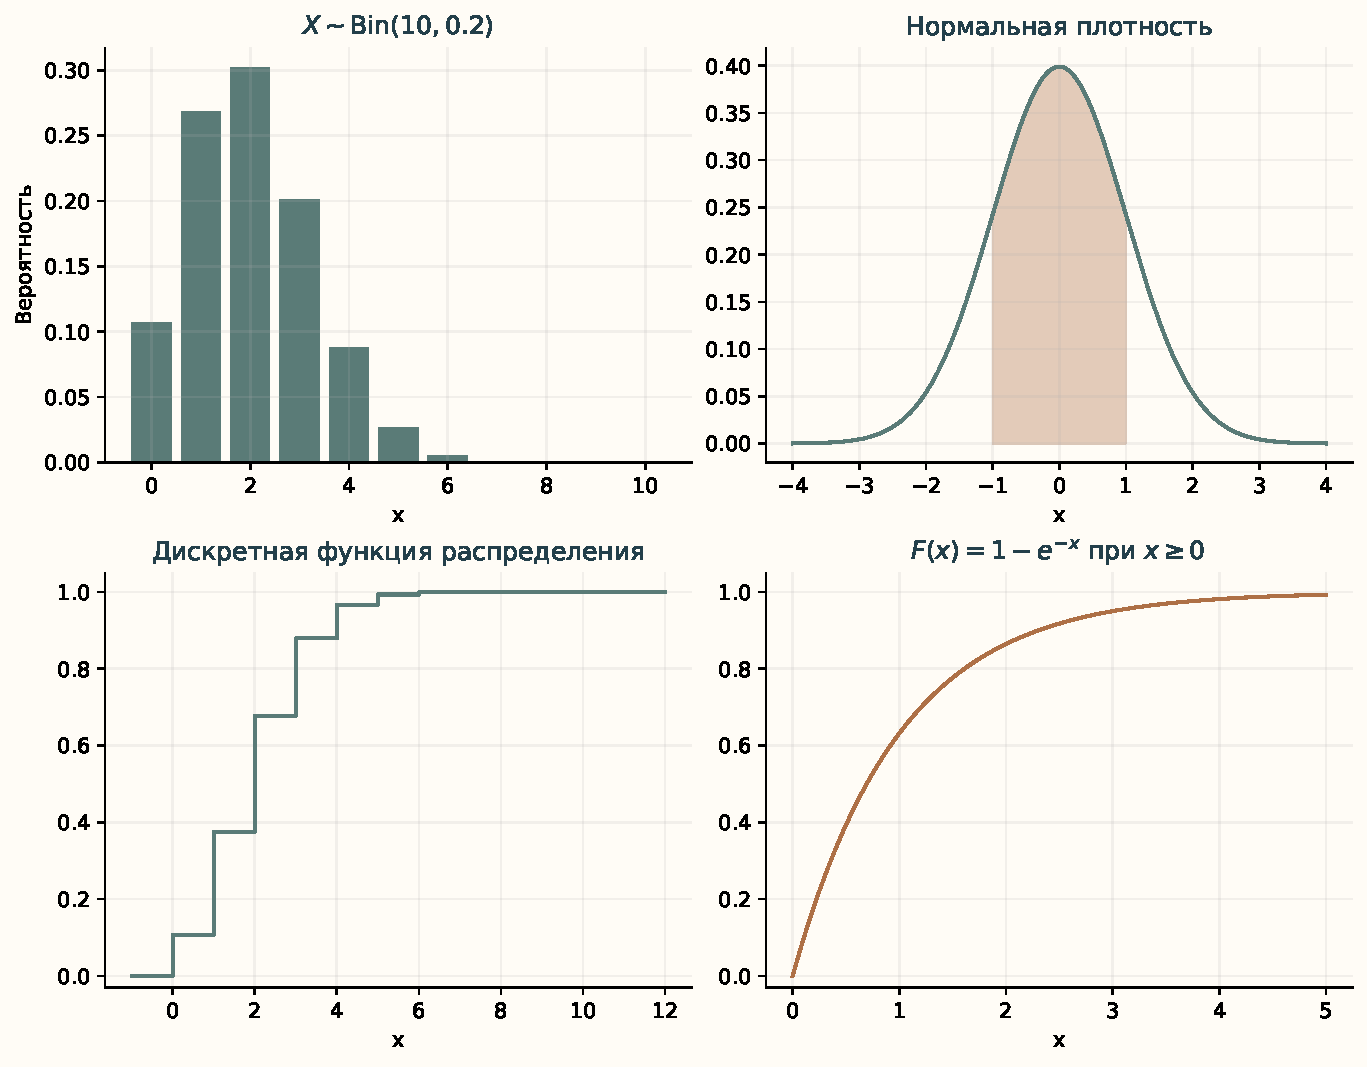
\includegraphics[width=\textwidth,height=.79\textheight,keepaspectratio]{images/atlas-random-variables.pdf}\par\small Дискретное распределение, плотность и функция распределения\end{center}\end{minipage}\par
\Needspace{7\baselineskip}\section*{Задачи}
\begingroup\setlength{\parskip}{1pt}
\noindent\begin{minipage}[t]{\linewidth}\textbf{37.1.} Величина принимает значения \(-1,0,2\) с вероятностями \(c,2c,c\). Найди \(c\).\par\end{minipage}\par
\noindent\begin{minipage}[t]{\linewidth}\textbf{37.2.} Для предыдущей величины запиши \(F_X(t)\).\par\end{minipage}\par
\noindent\begin{minipage}[t]{\linewidth}\textbf{37.3.} Для тех же значений и вероятностей найди \(\mathbb EX\) и \(\operatorname{Var}X\).\par\end{minipage}\par
\noindent\begin{minipage}[t]{\linewidth}\textbf{37.4.} Плотность равна \(cx\) на \([0,2]\) и нулю вне него. Найди \(c\) и \(\mathbb P(1<X<2)\).\par\end{minipage}\par
\noindent\begin{minipage}[t]{\linewidth}\textbf{37.5.} Для плотности предыдущей задачи найди среднее и дисперсию.\par\end{minipage}\par
\par\addvspace{5pt}\begin{lrbox}{\CatFlowBox}\begin{minipage}[t]{\linewidth}
\setlength{\parskip}{5pt}\setlength{\columnsep}{4.5mm}\setlength{\intextsep}{0pt}
\begin{wrapfigure}[10]{r}{54mm}

\includegraphics[width=54mm,height=58mm,keepaspectratio]{images/unique/art-176.png}
\end{wrapfigure}
\textbf{37.6.} Если у \(X\) есть плотность, чему равна \(\mathbb P(X=1)\)? Может ли \(f_X(1)>1\)?\par

\textbf{37.7.} Для \(X\sim\operatorname{Bern}(\dfrac15)\) найди среднее и дисперсию.\par

\textbf{37.8.} Для \(X\sim\operatorname{Bin}(10,\dfrac15)\) найди \(\mathbb P(X=0)\), среднее и дисперсию.\par

\textbf{37.9.} Независимые попытки успешны с вероятностью \(\dfrac14\). Для номера первого успеха найди вероятность \(X=3\) и среднее.\par
\par\WFclear\end{minipage}\end{lrbox}%
\ifdim\dimexpr\ht\CatFlowBox+\dp\CatFlowBox\relax<64mm\dp\CatFlowBox=\dimexpr64mm-\ht\CatFlowBox\relax\fi%
\noindent\usebox{\CatFlowBox}\par\addvspace{5pt}

\noindent\begin{minipage}[t]{\linewidth}\textbf{37.10.} Для \(X\sim\operatorname{Pois}(2)\) найди \(\mathbb P(X=0)\), \(\mathbb P(X=2)\), среднее и дисперсию.\par\end{minipage}\par
\noindent\begin{minipage}[t]{\linewidth}\textbf{37.11.} Автобус в учебной модели приходит через время \(X\sim\operatorname U[0,12]\). Найди \(\mathbb P(X>9)\), среднее и дисперсию.\par\end{minipage}\par
\noindent\begin{minipage}[t]{\linewidth}\textbf{37.12.} Для \(X\sim\operatorname{Exp}(2)\) найди \(\mathbb P(X>1)\), среднее и дисперсию.\par\end{minipage}\par
\noindent\begin{minipage}[t]{\linewidth}\textbf{37.13.} Для \(X\sim\operatorname N(10,4)\) вырази \(\mathbb P(8<X<12)\) через \(\Phi\).\par\end{minipage}\par
\noindent\begin{minipage}[t]{\linewidth}\textbf{37.14.} Если \(\mathbb EX=3\), \(\operatorname{Var}X=2\), найди среднее и дисперсию \(Y=4-2X\).\par\end{minipage}\par
\noindent\begin{minipage}[t]{\linewidth}\textbf{37.15.} Независимые \(X,Y\) имеют дисперсии \(2,5\). Найди дисперсию \(X+Y\) и \(X-Y\).\par\end{minipage}\par
\noindent\begin{minipage}[t]{\linewidth}\textbf{37.16.} Величина \(X\) имеет дисперсию \(3\). Найди дисперсию \(X+X\) и объясни, почему нельзя просто сложить две дисперсии.\par\end{minipage}\par
\noindent\begin{minipage}[t]{\linewidth}\textbf{37.17.} Для неотрицательной величины со средним \(6\) оцени сверху \(\mathbb P(X\ge30)\).\par\end{minipage}\par
\noindent\begin{minipage}[t]{\linewidth}\textbf{37.18.} Среднее равно \(10\), дисперсия \(4\). Оцени снизу \(\mathbb P(|X-10|<4)\).\par\end{minipage}\par
\noindent\begin{minipage}[t]{\linewidth}\textbf{37.19.} Независимые одинаково распределённые наблюдения имеют дисперсию \(9\). Какого \(n\) достаточно, чтобы по Чебышёву вероятность ошибки среднего не меньше \(0{,}3\) была не больше \(0{,}01\)?\par\end{minipage}\par
\noindent\begin{minipage}[t]{\linewidth}\textbf{37.20.}\starmark{} Докажи: если \(\operatorname{Var}X=0\), то \(X=\mathbb EX\) с вероятностью \(1\).\par\end{minipage}\par
\noindent\begin{minipage}[t]{\linewidth}\textbf{37.21.}\starmark{} Пусть \(X\) равновероятно принимает \(-1,0,1\), \(Y=X^2\). Найди ковариацию и докажи зависимость.\par\end{minipage}\par
\noindent\begin{minipage}[t]{\linewidth}\textbf{37.22.} Выведи формулу дисперсии среднего \(n\) независимых величин с общей дисперсией \(\sigma^2\).\par\end{minipage}\par
\noindent\begin{minipage}[t]{\linewidth}\textbf{37.23.}\starmark{} Докажи отсутствие памяти показательного распределения: при \(s,t\ge0\) найди \(\mathbb P(X>s+t\mid X>s)\).\par\end{minipage}\par
\noindent\begin{minipage}[t]{\linewidth}\textbf{37.24.} Докажи для событий \(A,B\): \(\operatorname{Cov}(1_A,1_B)=\mathbb P(A\cap B)-\mathbb P(A)\mathbb P(B)\).\par\end{minipage}\par
\endgroup
